\thispagestyle{empty}

%-------------------------------------------------------------------------------

\chapterimage{figures/chapter_head.pdf} % ------- This is stupid, but required -
\chapter{FIRST CHAPTER}
\label{chap:ch1}

Lorem ipsum dolor sit amet, consectetur adipiscing elit, sed do eiusmod
tempor incididunt ut labore et dolore magna aliqua. Ut enim ad minim
veniam, quis nostrud exercitation ullamco laboris nisi ut aliquip ex ea
commodo consequat. Duis aute irure dolor in reprehenderit in voluptate
velit esse cillum dolore eu fugiat nulla pariatur. Excepteur sint
occaecat cupidatat non proident, sunt in culpa qui officia deserunt
mollit anim id est laborum.

%-------------------------------------------------------------------------------

\section{First Section}
\label{sec:sec1}

[YOUR TEXT]

\subsection{First SubSection}

[YOUR TEXT]

\hfill \\

%-------------------------------------------------------------------------------
% CITATION EXAMPLE

Citation example: \\
\citep{aki2002} \\
\citep{cauzzi2008} \\
\citep{danciu2010} \\

%-------------------------------------------------------------------------------
% EQUATION EXAMPLE

Equation example:

\begin{equation}
  f_0 = \frac{Vs}{4H}
  \label{eq:eq1}
\end{equation}

%-------------------------------------------------------------------------------
% FIGURE EXAMPLE

\newpage
\hfill \\

\begin{figure}[htbp]
  \centering
  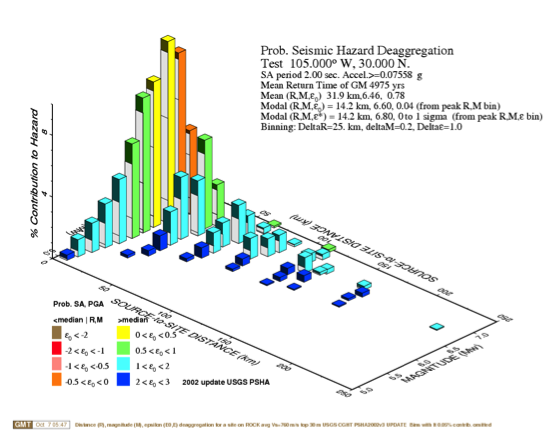
\includegraphics[width=10cm]{figures/Example.png}
  \caption{[CAPTION TEXT]}
  \label{fig:ex1}
\end{figure}

%-------------------------------------------------------------------------------
% TABLE EXAMPLE

\hfill \\

\begin{table}[htbp]
  \centering
  \begin{tabular}{lccc}
  \hline
  \rowcolor{lightgray}
  \bf{Heading 1} & \bf{Heading 2} & \bf{Heading 3} & \bf{Heading 4} \\
  \hline
  Text & 10 & 10 & 10 \\
  Text & 10 & 10 & 10 \\
  Text & 10 & 10 & 10 \\
  \hline
  \end{tabular}
  \caption{[CAPTION TEXT]}
  \label{tab:tab1}
\end{table}

%-------------------------------------------------------------------------------
% CODE EXAMPLE

\hfill \\

\lstset{frameround=fttt}
\lstset{backgroundcolor=\color{lightgray}}

\begin{lstlisting}[frame=trBL,caption={[CAPTION TEXT]},label=cod1]
  #!/bin/bash
  for file in *.txt
    do
    echo $file
  done
\end{lstlisting}
